\documentclass[a4paper,12pt]{report}
\addtolength{\oddsidemargin}{-1.cm}
\addtolength{\textwidth}{2cm}
\addtolength{\topmargin}{-2cm}
\addtolength{\textheight}{3.5cm}
\newcommand{\HRule}{\rule{\linewidth}{0.5mm}}
\makeindex


\usepackage[pdftex]{graphicx}
\usepackage{makeidx}
\usepackage{hyperref}
\hypersetup{
    colorlinks=true,
    linkcolor=blue,
    filecolor=magenta,      
    urlcolor=cyan,
}


% define the title
\author{Group6_a}
\title{ Assignment 1 Report}
\begin{document}
\setlength{\parskip}{6pt}

% generates the title
\begin{titlepage}

\begin{center}
% Upper part of the page       

\includegraphics[width=1\textwidth]{./up-logo.jpg}\\[0.4cm]    
\textsc{\LARGE Department of Computer Science}\\[1.5cm]
\textsc{\Large COS 301 - Software Engineering}\\[0.5cm]
% Title
\HRule \\[0.4cm]
{ \huge \bfseries COS 301 - Mini Project}\\[0.4cm]
\HRule \\[0.4cm]
% Author and supervisor
\begin{minipage}{0.4\textwidth}
\begin{flushleft} \large
\emph{Author:}\\
Hanrich {Potgieter}
\end{flushleft}
\end{minipage}
\begin{minipage}{0.4\textwidth}
\begin{flushright} \large
\emph{Student number:} \\
u12287343
\end{flushright}
\end{minipage}
\begin{minipage}{0.4\textwidth}
\begin{flushleft} \large
Chris {Cloete}
\end{flushleft}
\end{minipage}
\begin{minipage}{0.4\textwidth}
\begin{flushright} \large
\emph{} \\
u13029721
\end{flushright}
\end{minipage}
\begin{minipage}{0.4\textwidth}
\begin{flushleft} \large
Jason Richard {Evans}
\end{flushleft}
\end{minipage}
\begin{minipage}{0.4\textwidth}
\begin{flushright} \large
\emph{} \\
u13032608
\end{flushright}
\end{minipage}
\begin{minipage}{0.4\textwidth}
\begin{flushleft} \large
Kale-ab {Tessera}
\end{flushleft}
\end{minipage}
\begin{minipage}{0.4\textwidth}
\begin{flushright} \large
\emph{} \\
u13048423
\end{flushright}
\end{minipage}
\begin{minipage}{0.4\textwidth}
\begin{flushleft} \large
Lelethu {Zazaza}
\end{flushleft}
\end{minipage}
\begin{minipage}{0.4\textwidth}
\begin{flushright} \large
\emph{} \\
u13028023
\end{flushright}
\end{minipage}
\begin{minipage}{0.4\textwidth}
\begin{flushleft} \large
Goodness {Adegbenro}
\end{flushleft}
\end{minipage}
\begin{minipage}{0.4\textwidth}
\begin{flushright} \large
\emph{} \\
u13046412
\end{flushright}
\end{minipage}
\begin{minipage}{0.4\textwidth}
\begin{flushleft} \large
Herman Willem {Keuris}
\end{flushleft}
\end{minipage}
\begin{minipage}{0.4\textwidth}
\begin{flushright} \large
\emph{} \\
u13037618
\end{flushright}
\end{minipage}
\vfill
% Bottom of the page
{\large \today}
\end{center}
\end{titlepage}
\footnotesize
<<<<<<< HEAD
%%
%%  University of Pretoria - Declaration of Originality
%%  Version: S4726/09 (amended 2010-07-23)
%%

\newpage

\thispagestyle{empty}
{
\renewcommand{\baselinestretch}{1}
\sffamily
\begin{center}
\textbf{\Large DECLARATION OF ORIGINALITY}
\end{center}
\begin{center}
\textbf{\large UNIVERSITY OF PRETORIA}
\end{center}

The University of Pretoria places great emphasis upon integrity and
ethical conduct in the preparation of all written work submitted for
academic evaluation.

While academic staff teach you about referencing techniques and how to
avoid plagiarism, you too have a responsibility in this regard. If you
are at any stage uncertain as to what is required, you should speak to
your lecturer before any written work is submitted.

You are guilty of plagiarism if you copy something from another
author's work (e.g. a book, an article or a website) without
acknowledging the source and pass it off as your own. In effect you
are stealing something that belongs to someone else. This is not only
the case when you copy work word-for-word (verbatim), but also when
you submit someone else's work in a slightly altered form (paraphrase)
or use a line of argument without acknowledging it. You are not
allowed to use work previously produced by another student. You are
also not allowed to let anybody copy your work with the intention of
passing if off as his/her work.

Students who commit plagiarism will not be given any credit for
plagiarised work. The matter may also be referred to the Disciplinary
Committee (Students) for a ruling. Plagiarism is regarded as a serious
contravention of the University's rules and can lead to expulsion from
the University.

The declaration which follows must accompany all written work
submitted while you are a student of the University of Pretoria. No
written work will be accepted unless the declaration has been
completed and attached.

\begin{center}
\begin{tabular}{ll}
                        &                             \\
 Full names of student: & \makebox[3.5in]{\hrulefill} \\ \\
 Student number:        & \makebox[3.5in]{\hrulefill} \\ \\
 Topic of work:         & \makebox[3.5in]{\hrulefill} \\ \\
\end{tabular}
\end{center}

\textbf{Declaration}
\begin{enumerate}
\item I understand what plagiarism is and am aware of the University's
  policy in this regard.
\item I declare that this assignment report is my own original work.
  Where other people's work has been used (either from a printed source,
  Internet or any other source), this has been properly acknowledged and
  referenced in accordance with departmental requirements.
\item I have not used work previously produced by another student or any
  other person to hand in as my own.
\item I have not allowed, and will not allow, anyone to copy my work with
  the intention of passing it off as his or her own work.
\end{enumerate}

\vspace*{1cm}

SIGNATURE: \makebox[3in]{\hrulefill} \quad DATE: \makebox[1.5in]{\hrulefill}
}

\newpage


=======
%%
%%  University of Pretoria - Declaration of Originality
%%  Version: S4726/09 (amended 2010-07-23)
%%

\newpage

\thispagestyle{empty}
{
\renewcommand{\baselinestretch}{1}
\sffamily
\begin{center}
\textbf{\Large DECLARATION OF ORIGINALITY}
\end{center}
\begin{center}
\textbf{\large UNIVERSITY OF PRETORIA}
\end{center}

The University of Pretoria places great emphasis upon integrity and
ethical conduct in the preparation of all written work submitted for
academic evaluation.

While academic staff teach you about referencing techniques and how to
avoid plagiarism, you too have a responsibility in this regard. If you
are at any stage uncertain as to what is required, you should speak to
your lecturer before any written work is submitted.

You are guilty of plagiarism if you copy something from another
author's work (e.g. a book, an article or a website) without
acknowledging the source and pass it off as your own. In effect you
are stealing something that belongs to someone else. This is not only
the case when you copy work word-for-word (verbatim), but also when
you submit someone else's work in a slightly altered form (paraphrase)
or use a line of argument without acknowledging it. You are not
allowed to use work previously produced by another student. You are
also not allowed to let anybody copy your work with the intention of
passing if off as his/her work.

Students who commit plagiarism will not be given any credit for
plagiarised work. The matter may also be referred to the Disciplinary
Committee (Students) for a ruling. Plagiarism is regarded as a serious
contravention of the University's rules and can lead to expulsion from
the University.

The declaration which follows must accompany all written work
submitted while you are a student of the University of Pretoria. No
written work will be accepted unless the declaration has been
completed and attached.

\begin{center}
\begin{tabular}{ll}
                        &                             \\
 Full names of students: & \makebox[3.5in]{\hrulefill} \\ \\
 Student numbers:        & \makebox[3.5in]{\hrulefill} \\ \\
 Topic of work:         & \makebox[3.5in]{\hrulefill} \\ \\
\end{tabular}
\end{center}

\textbf{Declaration}
\begin{enumerate}
\item I understand what plagiarism is and am aware of the University's
  policy in this regard.
\item I declare that this assignment report is my own original work.
  Where other people's work has been used (either from a printed source,
  Internet or any other source), this has been properly acknowledged and
  referenced in accordance with departmental requirements.
\item I have not used work previously produced by another student or any
  other person to hand in as my own.
\item I have not allowed, and will not allow, anyone to copy my work with
  the intention of passing it off as his or her own work.
\end{enumerate}

\vspace*{1cm}

SIGNATURES: \makebox[3in]{\hrulefill} \quad DATE: \makebox[1.5in]{\hrulefill}
}

\newpage


>>>>>>> c9c34b47029f66b93ead74067c518a6171377c84

\normalsize

\renewcommand{\thesection}{\arabic{section}}
\newpage
\begin{center}
\textsc{\LARGE Software Requirements Specification and Technology Neutral Process Design}\\[1.5cm]
\textsc{\Large Buzz Space Discussions/Mini Project}\\[0.5cm]
Version: Version 0.2 Alpha 
For further references see \href{http://www.sharelatex.com}{gitHub}.
\today
\end{center}
\tableofcontents{}
For further references see \href{http://www.sharelatex.com}{gitHub}.
\section{Functional requirements}
\subsection{Introduction}
We use this document to give a high level overview of the buzz space discussion board. We have identified the various components. Our purpose is to create a dynamic and scalable solution. We also want to include an Achievement system that rewards users for using the discussion board. This document will inform you how we well achieve a system that is both scalable and pluggable.
\subsection{Use case prioritiation}
\textbf{Critical} 
\begin{itemize}
  \item Login System.
	\begin{center}
  	% 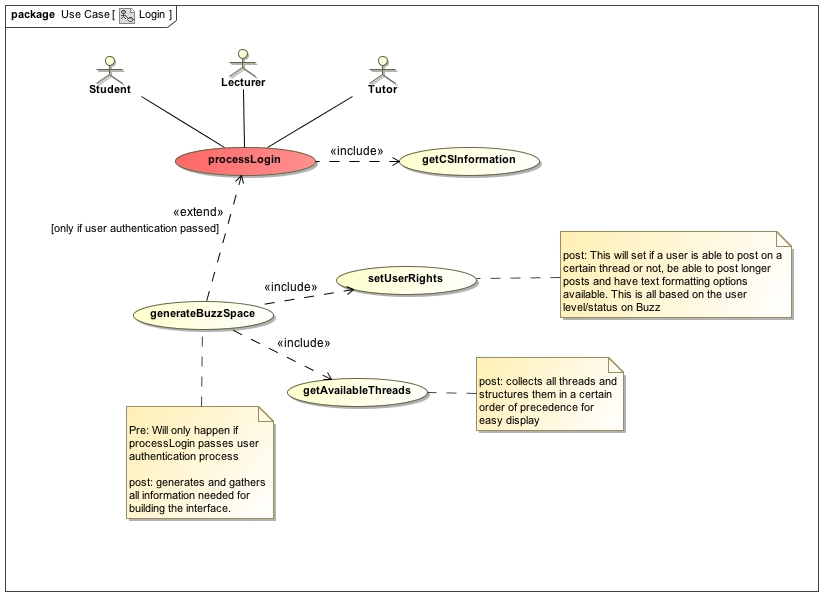
\includegraphics[width=1\textwidth] {../Functional_Requirements_DIagrams/UseCases/UseCase_Login.jpg}\\[0.4cm]    
	\end{center}
  \item Logout System
	\begin{center}
  	% 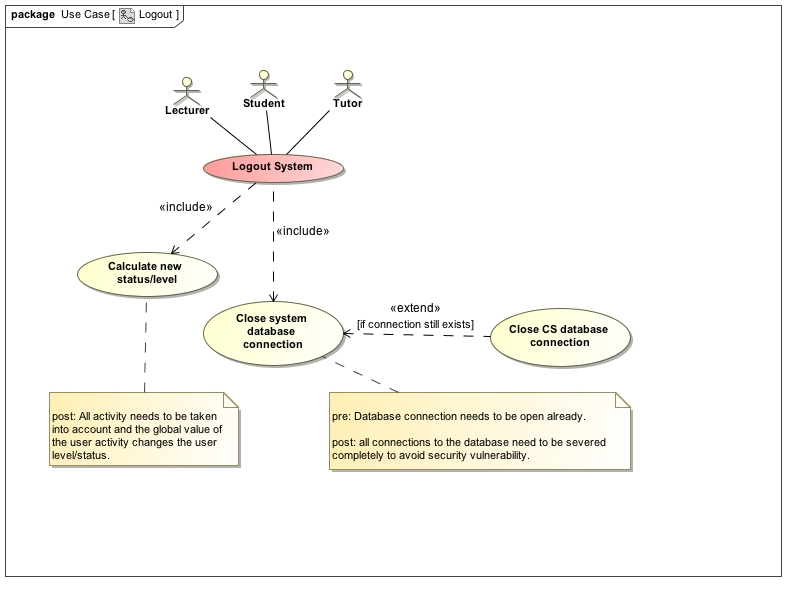
\includegraphics[width=1\textwidth]{../Functional_Requirements_DIagrams/UseCases/UseCase_Logout.jpg}\\[0.4cm]    
	\end{center}	
  \item Creation of a Buzz thread.
    \item CRUD OWN posts(Creating,Reading; Updating; Deleting).
	\begin{center}
  	% 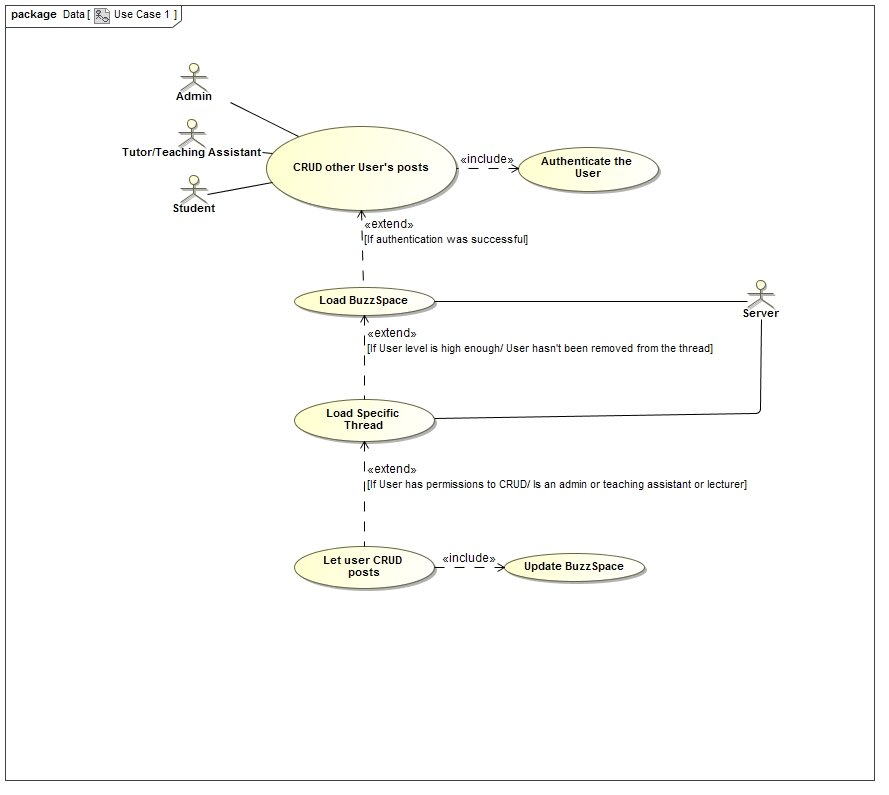
\includegraphics[width=1\textwidth]{../Functional_Requirements_Diagrams/UseCases1,2,3 - Kale-ab Tessera/UseCase1.jpg}\\[0.4cm]    
	\end{center}
\item CRUD Other people's posts 
	\begin{center}
  	% 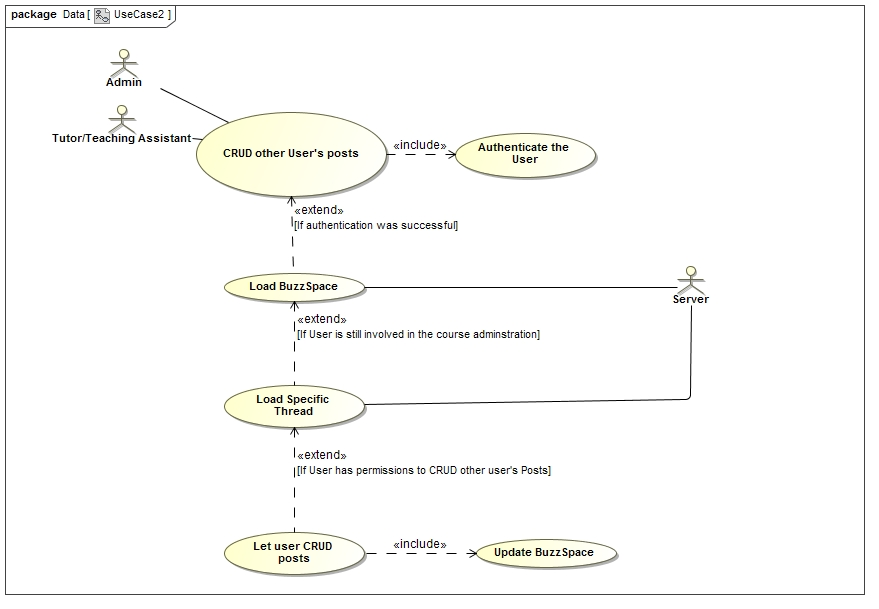
\includegraphics[width=1\textwidth]{../Functional_Requirements_Diagrams/UseCases1,2,3 - Kale-ab Tessera/UseCase2.jpg}\\[0.4cm]    
	\end{center}\end{itemize} 

\textbf{Important} 
\begin{itemize}
  \item Content Management (By higher level users and Administrators).
  \item User Restriction based on level.
	\begin{center}
  	% 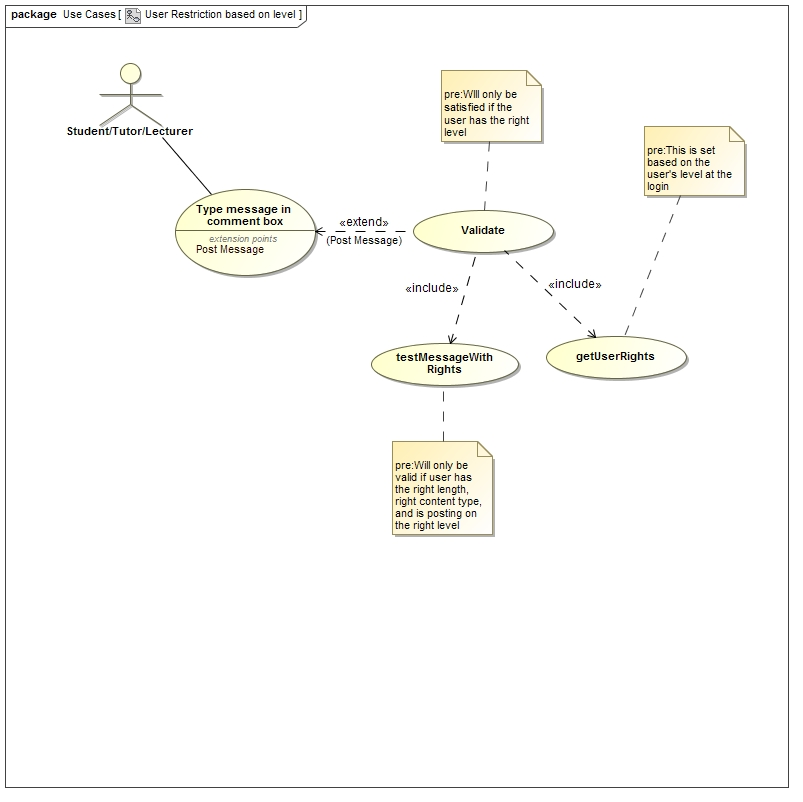
\includegraphics[width=1\textwidth]{../Functional_Requirements_DIagrams/UseCases/use_case_message_Restriction.jpg}\\[0.4cm]    
	\end{center}	
  \item Automatic update of user status.
  \item Semi-Automatic evaluation of posts.
  \item Gathering and analization of statistical information.
	\begin{center}
  	% 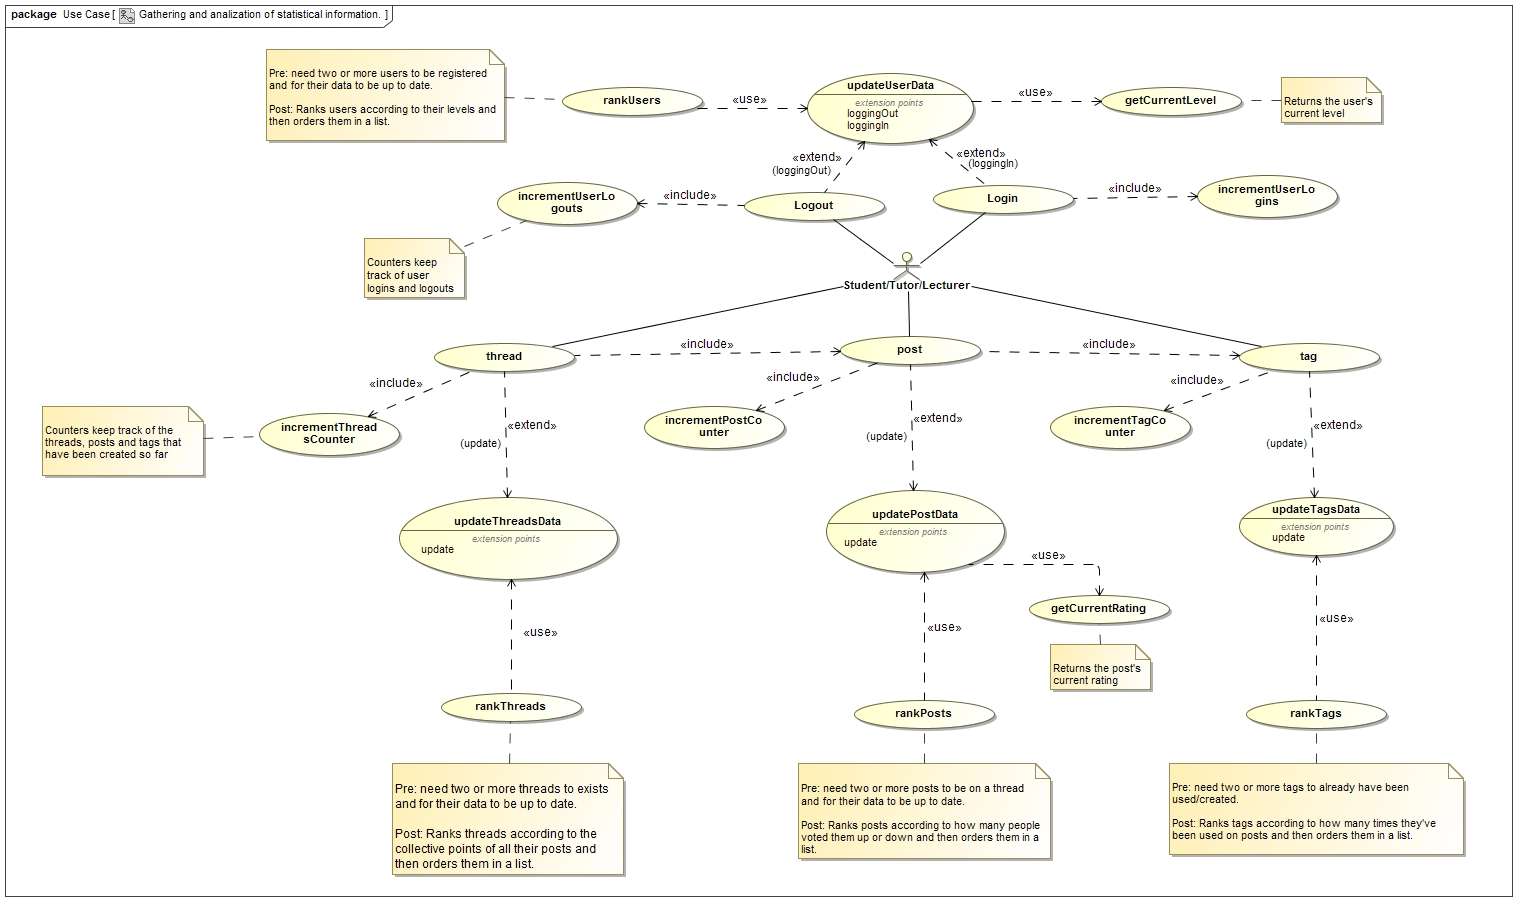
\includegraphics[width=1\textwidth]{../Functional_Requirements_DIagrams/UseCases/UseCase_StatisticalInformation.jpg}\\[0.4cm]    
	\end{center}
  \item Social tagging system on threads (and posts).
	\begin{center}
  	% 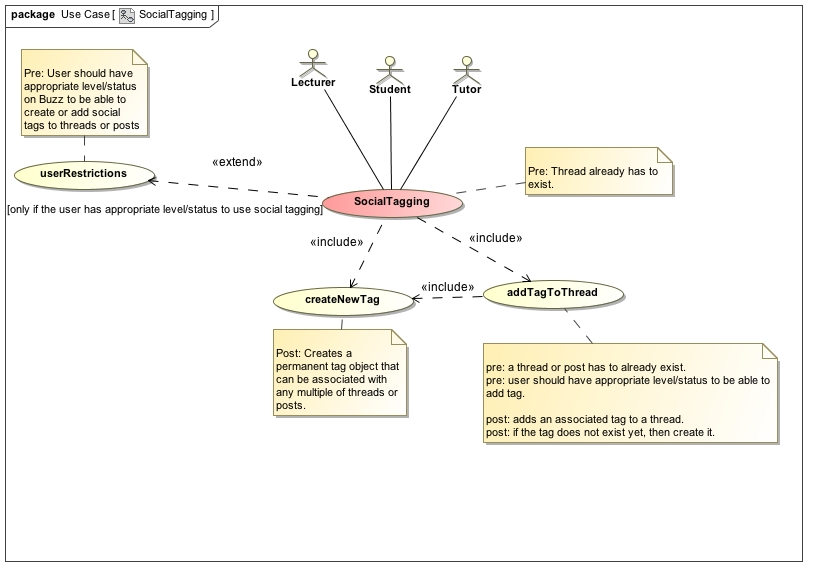
\includegraphics[width=1\textwidth]{../Functional_Requirements_DIagrams/UseCases/UseCase_SocialTagging.jpg}\\[0.4cm]    
	\end{center}
  \item Searching and filtering of threads.
	\begin{center}
  	% 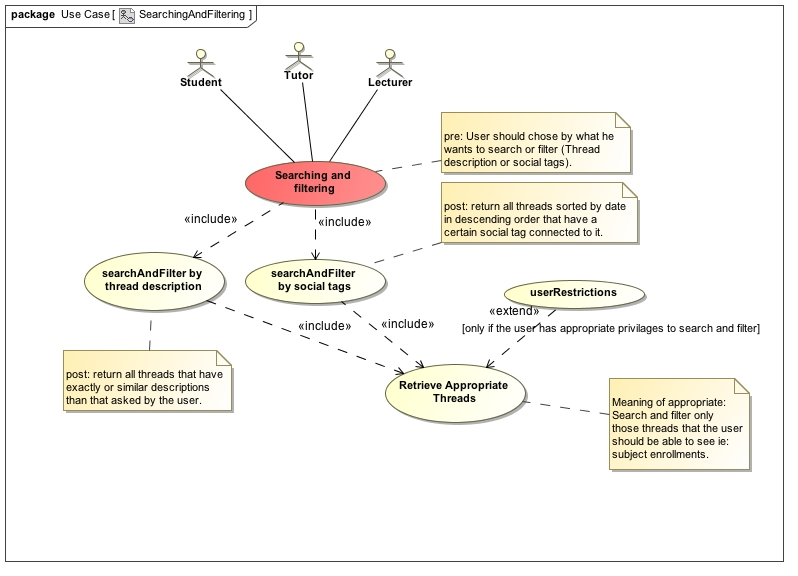
\includegraphics[width=1\textwidth]{../Functional_Requirements_DIagrams/UseCases/UseCase_SearchingAndFiltering.jpg}\\[0.4cm]    
	\end{center}
  \item Format code in an easy to view/edit layout.
	\begin{center}
  	% 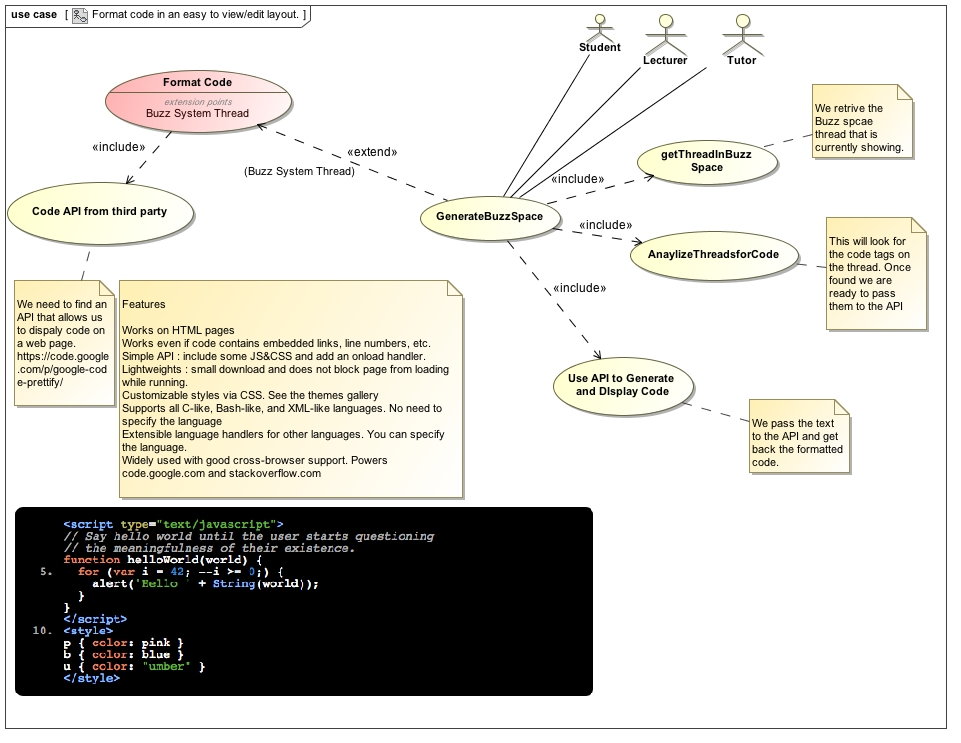
\includegraphics[width=1\textwidth]		{../Functional_Requirements_DIagrams/UseCases/UseCase_FormatCode.jpg}\\[0.4cm]    
	\end{center}
\end{itemize}
\textbf{Nice-To-Have} 
\begin{itemize}
  \item Keeping track of who read what (ie. Message Highlighting).
 	\begin{center}
  	% 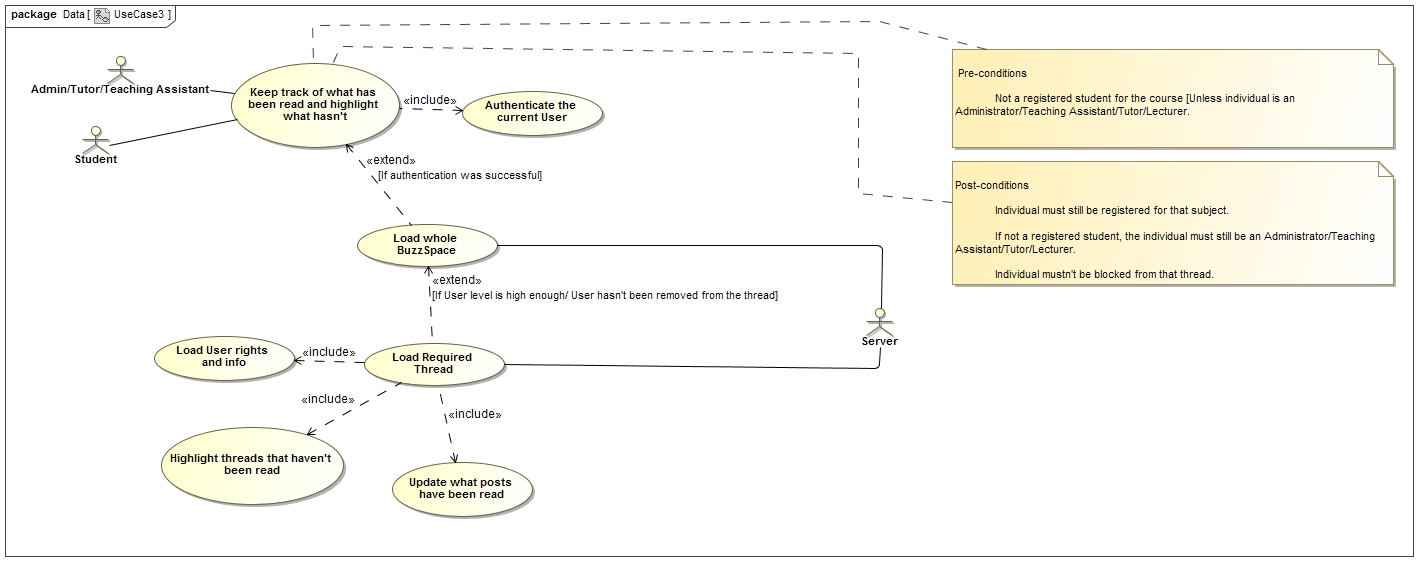
\includegraphics[width=1\textwidth]{../Functional_Requirements_Diagrams/UseCases1,2,3 - Kale-ab Tessera/UseCase3.jpg}\\[0.4cm]    
	\end{center} 
  \item Semi-Automatic functionality for generating thread summaries.
  \item Text formatting functionality based on user level.
  \item Self organization functionality.
  \item Automatic plagiarism checking system.
  \item Semi-Automatic detection of netiquette rule violations.
  \item Have functionality to vote for and evaluate posts.
\begin{center}
  	% 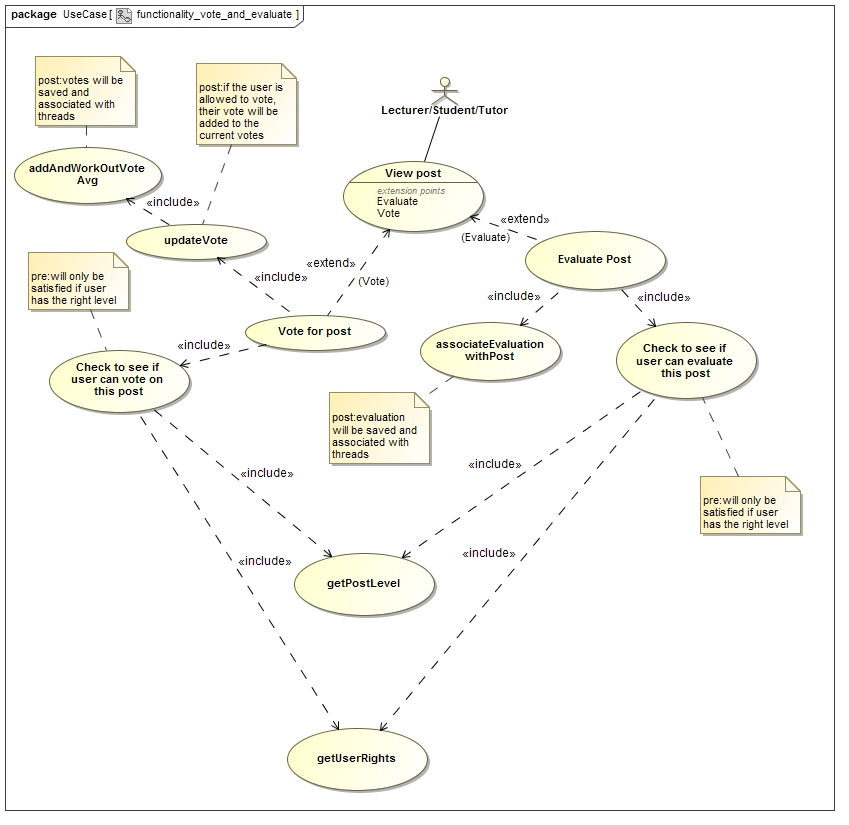
\includegraphics[width=1\textwidth]{../Functional_Requirements_DIagrams/UseCases/functionality_vote_and_evaluate.jpg}\\[0.4cm]    
	\end{center}	
\end{itemize}
\subsection{Use case/Service contracts}

\textbf {1. CRUD (Creating, reading, updating, deleting posts) OWN posts}
\begin{itemize}
    \item\textbf{Pre-conditions}

	{ Student is not registered for a course [Unless he/she is a Teaching Assistant/Tutor/Lecturer/Admin.}

	{Student must be a high enough level to participate in the thread. [Unless he/she is given permission by an Admin or Lecturer.}
 
    \item\textbf{Post-conditions }

	{Student is still registered for the course.}

	{Student hasn't been blocked from the thread.}

	{Student level must still be high enough to participate in the thread.} 

    \item\textbf{Request and Results Data Structure} 

\end{itemize}
\textbf {2. CRUD (Creating, reading, updating, deleting posts) OTHER People's posts}
\begin{itemize}
    \item\textbf{Pre-conditions}

	{Not an adminstrator. [Unless he/she is a Teaching Assistant/Tutor/Lecturer]}

	{Not a high enough level. [Unless given permission by the System Adminstrator]}
 
    \item\textbf{Post-conditions }

	{Individual must still be an Administrator/Teaching Assistant/Tutor/Lecturer.}

	{Level must still be high enough to allow an individual to CRUD other people's posts.}

	{Individual mustn't be blocked from that thread.}


    \item\textbf{Request and Results Data Structure} 

\end{itemize}
\textbf {3. Keep track of what has been read and highlight all unread messages in a particular thread}
\begin{itemize}
    \item\textbf{Pre-conditions}

	{Not a registered student for the course [Unless individual is an Administrator/Teaching Assistant/Tutor/Lecturer.}

    \item\textbf{Post-conditions }

	{Individual must still be registered for that subject.}

	{If not a registered student, the individual must still be an Administrator/Teaching Assistant/Tutor/Lecturer.}

	{Individual mustn't be blocked from that thread.}


    \item\textbf{Request and Results Data Structure} 

\end{itemize}

\subsection{Required functionality}

\subsection{Process specification}
\subsection{Domain Model}
	\begin{center}
  	% 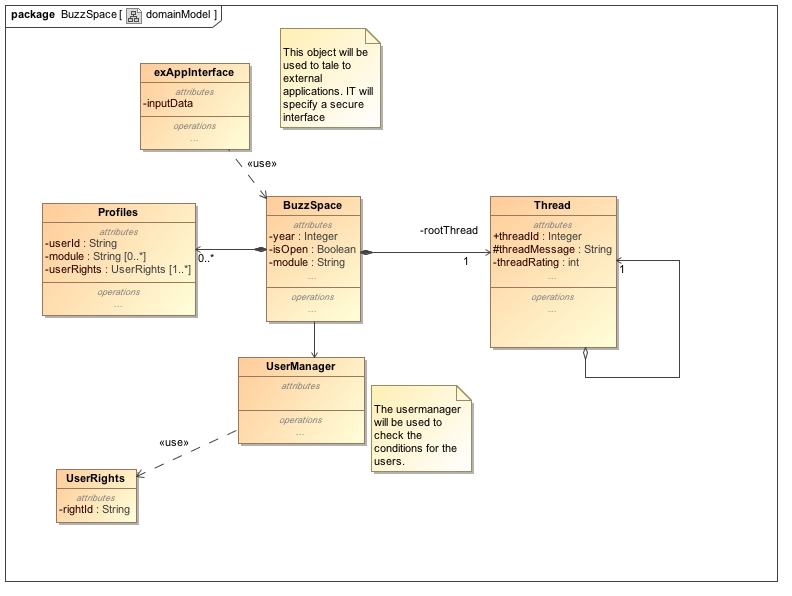
\includegraphics[width=1\textwidth]		{../Functional_Requirements_DIagrams/DomainModel/DomainModel.jpg}\\[0.4cm]    
	\end{center}
\index{Vision}
\newpage


\bibliography{myrefs}{} % expects file "myrefs.bib"
\bibliographystyle{ieeetr}
\end{document}